\ifsvnmulti
 \svnkwsave{$RepoFile: xiong/blog/DiffMat.tex $}
 \svnidlong {$HeadURL: svn://zero.physics.gatech.edu/siminos/xiong/blog/DiffMat.tex $}
 {$LastChangedDate: 2016-06-25 12:05:51 -0400 (Sat, 25 Jun 2016) $}
 {$LastChangedRevision: 4981 $} {$LastChangedBy: xiong $}
 \svnid{$Id: DiffMat.tex 4981 2016-06-25 16:05:51Z xiong $}
\fi

%%%%%%%%%%%%%%%%%%%%% Differential matrix and Fast Fourier Transform%%%%%%%%%%%%%%%%%%%%%%%%%%%%%%%%%%%

\section{Differential matrix and FFT}
\label{sect:DiffMat}


\begin{description}

\item[2013-09-09 Xiong]
I am reading N.~Trefethen's book \texttt{Spectral Methods in Matlab}, and
the following is what I learnt.
\end{description}



\subsection{Differential matrix}
The basic idea of \textit{differential matrix} is to use inverse discrete Fourier
transform to interpolate a set of points, and then get the derivative at those
points.

First, let's focus on the Semidiscrete Fourier transform. When discretizing a
continuous equation, we choose a point set
${x_{j}:j=h*n,n=..., -1,0,1,...}$ which is equally spaced in x-axis and there
is a field at those points $v_j$. Right now
we assume there is no boundary in the x-axis. The Semidiscrete Fourier transform
is defined as:

\begin{equation}
 \hat{v}(k)=h\sum_{j=-\infty}^{\infty}e^{-ikx_{j}}v_{j} \quad k\in  [-\pi/h,\pi/h]
\end{equation}

Note that the wavenumber $k$ is restricted in $[-\pi/h,\pi/h]$, which comes from the
consideration of \texttt{aliasing}, since $k$ and $k+2\pi/h$ give the same mode.

The Inverse Discrete Fourier transform is defined as:
\begin{equation}
 v_{j}=\frac{1}{2\pi}\int_{-\pi/h}^{\pi/h}e^{ikx_{j}}\hat{v}(k)dk \quad j\in \mathbb{Z}
\end{equation}

From this description, it is clear that discretization of coordinate
domain will lead to the Fourier domain to be bounded.

So, what if the coordinate space is discretized and bounded at the same time? Let's
consider a periodic function $v(x)$ with period $2\pi$, and the number of gird points in
the interval $[0,2\pi]$ is $N$:

\begin{equation}
 \frac{\pi}{h}=\frac{N}{2}
\end{equation}

Now we define the Discrete Fourier transform of $v_{j}$:
\begin{equation}
\label{eq:xiong_dft}
 \hat{v}_{k}=h\sum_{j=1}^{N}e^{-ikx_{j}}v_{j} \quad k=-\frac{N}{2}+1,\dots ,\frac{N}{2}
\end{equation}

Here, wavenumber $k$ is not only bounded but also discretized, because we want to make
sure that very term in the right side of \eqref{eq:xiong_dft} has a period $2\pi$.
The corresponding Inverse Discrete Fourier transform is:
\begin{equation}
\label{eq:xiong_idft}
 v_{j}=\frac{1}{2\pi}\sum_{k=-N/2+1}^{N/2}e^{ikx_{j}}\hat{v}_{k} \quad j=1,\dots ,N
\end{equation}

Our ultimate goal is to find an interpolant of points ${v_{j}:j=1,\dots ,N}$, and
\eqref{eq:xiong_idft} is just what we desire. The interpolant is given as:
\begin{equation}
\label{eq:xiong_interp_tm}
 P(x)=\frac{1}{2\pi}\sum_{k=-N/2+1}^{N/2}e^{ikx}\hat{v}_{k} \quad
 x\in [0,2\pi]=[0,hN]
\end{equation}
This function will return $P(x_{j})=v_{j}$. Equipped with such an interpolant, we can
write down the formula to approximate the derivatives at points ${x_{j}}$. But before
we that, interpolant \eqref{eq:xiong_interp_tm} should be modified slightly
to make it physically valid.

The derivative of mode $e^{iN/2*x}$ in \eqref{eq:xiong_interp_tm} is $iN/2*e^{iN/2*x}$,
which is $iN/2*e^{iN/2*x_{j}}=iN/2*(-1)^{j}$ at grid point $x_{j}$; however, this is
unphysical. The $k=N/2$ mode has maximal or minimal values at
the grid points, so it should have vanish derivative at grid points. This discrepancy
results from the asymmetrical summation limit in \eqref{eq:xiong_interp_tm}:
We use $k=N/2$ mode but discard $k=-N/2$ mode. To rescue formula
\eqref{eq:xiong_interp_tm}, we define $v_{-N/2}=v_{N/2}$ and extend the summation in
\eqref{eq:xiong_interp_tm} to mode $k=-N/2$ :

\begin{align}
\label{eq:xiong_interp}
 P(x)&=\frac{1}{2\pi}\sideset{}{'}\sum_{k=-N/2}^{N/2}e^{ikx}\hat{v}_{k} \quad
 x\in [0,2\pi]=[0,hN]  \\
 &=\frac{1}{2\pi}\sum_{k=-N/2+1}^{N/2-1}e^{ikx}\hat{v}_{k}+\frac{1}{2}
 (e^{i\frac{N}{2}x}+e^{-i\frac{N}{2}x})v_{\frac{N}{2}} \nonumber\\
 &=\frac{1}{2\pi}\sum_{k=-N/2+1}^{N/2-1}e^{ikx}\hat{v}_{k}+
 \cos(\frac{N}{2}x)v_{\frac{N}{2}} \nonumber
\end{align}

Where, the prime on the summation means only half of the modes
$k=N/2$ and $k=-N/2$ are taken into consideration.

Now we turn to Differential matrix. For every periodic function $v(x)$
with period $2\pi$, it satisfies
$v_{j}=v(x_{j})=\sum_{m=1}^{N}v_{m}\delta_{jm}$ at
 grid point $x_{j}=jh$, where the circular delta function is:
 \[
 \delta_{0j} =
  \begin{cases}
   1 & j\equiv 0 \pmod N \\
   0 & j\not\equiv 0 \pmod N
  \end{cases}
\]

The interpolant of delta function $\delta (j)$is

\begin{equation}
\label{eq:xiong_sn}
 S_{N}(x)=\frac{\sin (\frac{\pi x}{h})}{\frac{2\pi}{h}\tan (\frac{x}{2})}
\end{equation}

Thus, the interpolant of $v(x)$ at grid points ${x=jh,j=1,\dots ,N}$ is
\begin{equation}
\label{eq:xiong_px}
 P(x)=\sum_{m=1}^{N}v_{m}S_{N}(x-x_{m})
\end{equation}

The Spectral Differential matrix is defined:
$P^{'}(x)|_{x_{i}}=D_{i,j}v_{j}$ .
We can easily derive the form of Spectral Differential matrix from
\eqref{eq:xiong_sn} and \eqref{eq:xiong_px}:
\[
 D_{i,j}=
	 \begin{cases}
          \frac{1}{2}(-1)^{i-j}\cot \frac{(i-j)h}{2} & i\not\equiv j \pmod N  \\
          0 & i\equiv j \pmod N
         \end{cases}
\]


In the same way, we can define higher order spectral differential matrix.

By the way, if function $f(x)$ is periodic in range $[0,L]$, let $y=\frac{2\pi}{L}x$.
Then we can get the Spectral Differential matrix for $f(x)$: $\frac{2\pi}{L}D_{N}$,
where $D_{N}$ is the Spectral Differential matrix for a function with period $2\pi$,
which only depend on the number of discrete points.

\subsection{FFT}

\begin{description}
\item[2013-09-15 Xiong]
\end{description}



Suppose $v(x)$ is a periodic function in $[0,2\pi]$, now we have to numerical
methods to calcualate partial derivative $v_{x}(x_i)$, where $i=1,2,\dots , N$.

\begin{itemize}
 \item Toeplitz matrix.

 Toeplitz matrix refers to the Spectral Differential matrix in the the last section.

 Given $v(x_i)$, compute its Discrete Fourier Transform $\hat{v}_{k}$.

 Use Inverse Discrete Fourier Transform to interpolate $v(x)$:
 \[
 P(x)=\sum_{m=1}^{N}v_{m}S_{N}(x-x_{m})
\]

 Take the derivative of $P(x)$ at $x_{j}$,  $j=1,2,\dots , N$ to get the Spectral
 Differential matrix: $P^{'}(x)|_{x_{j}}=D_{i,j}v_{j}$. Then,
 $\mathbf{\partial v}=\mathbf{D_{n}}\mathbf{v}$. Here, $\mathbf{\partial v}$ is a vector
 whose components are the derivative of $v(x)$ at points $x_{j}, j=1,2,\dots , N$.

 \item FFT

 Let $\hat{v}$ and $\hat{\omega}$ be
 the Discrete Fourier Transform mode of $v$ and $\partial v$ respectively
 : $\hat{v}=\mathbf{fft}(v)$, $\hat{\omega}=\mathbf{fft}(\partial v)$.
 From equation \eqref{eq:xiong_interp}, we have
 relation $\hat{\omega}_{k}=ik\hat{v}_{k}$ for $k=-N/2+1,\dots , N/2-1$
 and $\hat{\omega}_{N/2}=0$.

 Therefore, the derivative of $v(x)$ at discrete points $x_{j} j=1,2,\dots , N$ is
 \begin{equation}
 \label{eq:xiong_fft}
  \mathbf{\partial v}=\mathbf{ifft}(i\cdot K\cdot \mathbf{fft(v)})
 \end{equation}

 where, $K=diag(-N/2+1,-N/2+2,\dots, N/2-1, 0)$. In formula \eqref{eq:xiong_fft},
 $\mathbf{fft(v)}$ and $\mathbf{ifft(v)}$ represent Fast Fourier Transform and
 Inverse Fast Fourier Transform respectively. In practice, we usually turn to
 well-matained Fast Fourier Transform packages, eg, \texttt{fft()} function in Matlab.
 However, the \texttt{fft()} function in Matlab has different wavenumbers order:
  \begin{equation}
  \label{eq:xiong_wavenumber_fft}
  k=0,1,2,\dots , N-1
 \end{equation}

 So, after aliasing \eqref{eq:xiong_wavenumber_fft} into interval $[-N/2+1,\dots,N/2]$,
 it becomes $k=0,1,\dots , N/2-1, N/2, -N/2+1,\dots, -1$. Also taking into accout
 $\hat{\omega}_{N/2}=0$, the diagonal matrix in \eqref{eq:xiong_fft} becomes
   \begin{equation}
  \label{eq:xiong_wavenumber_fft_matlab}
  K=diag(0,1,\dots, N/2-1, 0, -N/2+1,\dots, -1)
 \end{equation}

 I think this is the reason why Ruslan sets the wavenumber \texttt{k=[0:N/2-1 0 -N/2:-1:-1]'}
 in his matlab code in \texttt{siminos/matlab/ruslan}.

 \end{itemize}

 I tried these two methods to
 evolve \KS\ equation for periodic orbit $T10.25$. \refFig{fig:xiong_sdmfft_dif} shows that
 the numerical difference of these two methods is less than $10^{-10}$ for one period.

 \begin{figure}[h]
 \centering
 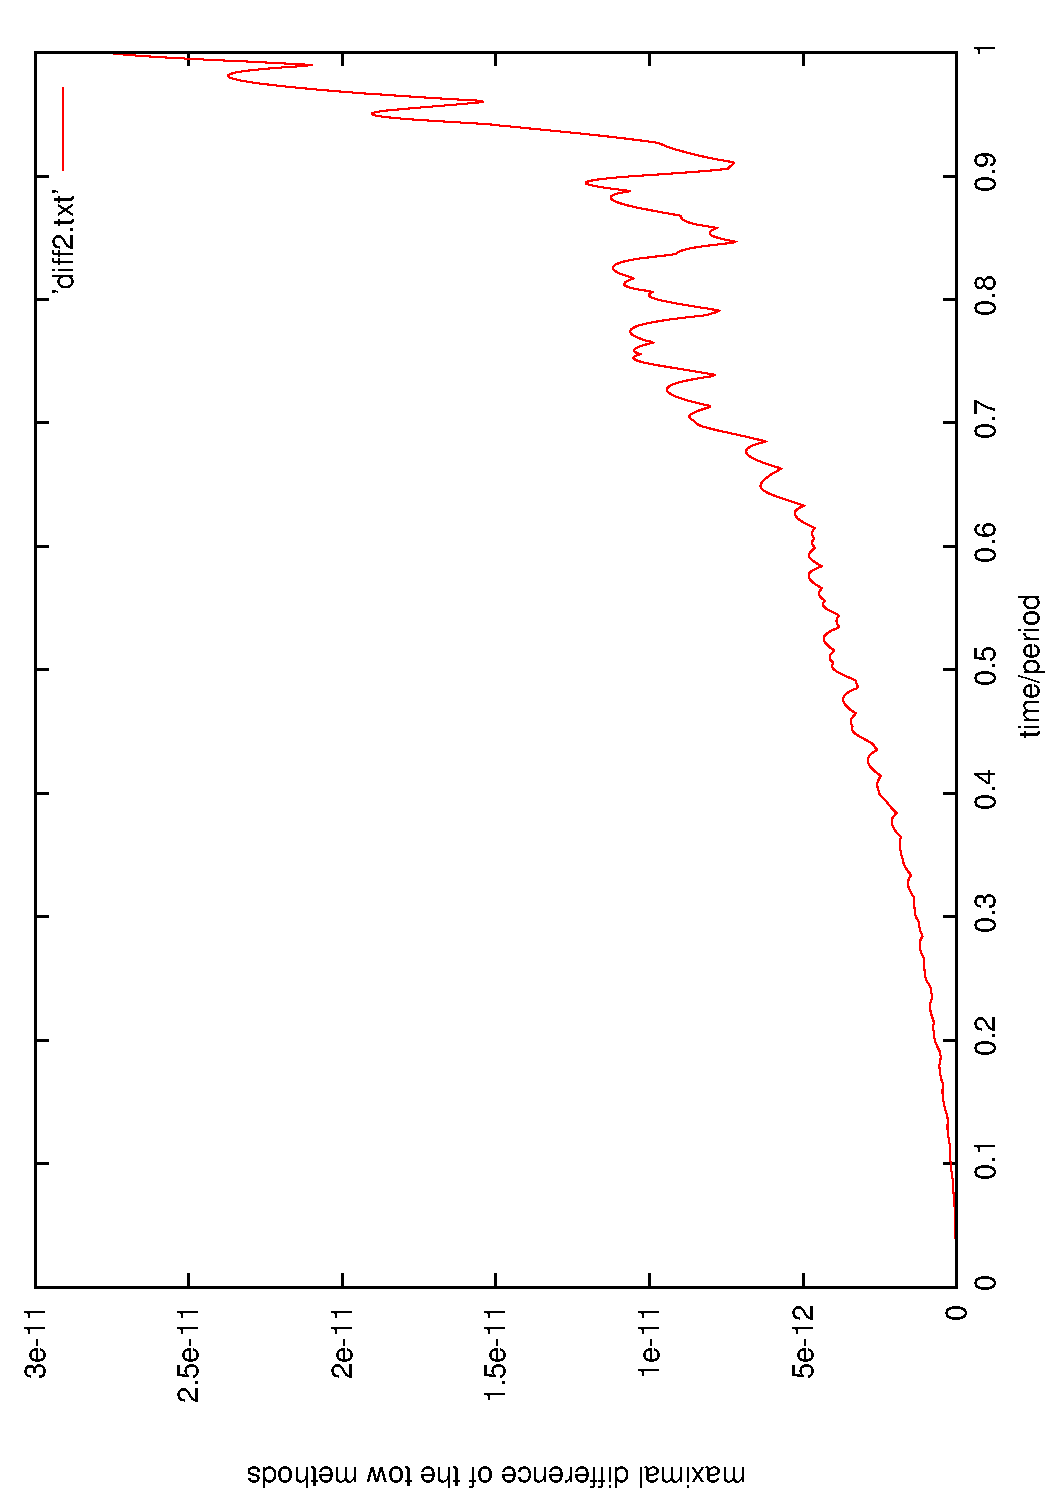
\includegraphics[angle=-90,width=0.5\textwidth]{diff-eps-converted-to.pdf}
 \caption{the maximal difference of the fourier modes for one period along the periodic orbit
  $T10.25$.}
 \label{fig:xiong_sdmfft_dif}
\end{figure}

\clearpage

%%%----------------------------------------------------------------------------
\subsection{Chebyshev Differential Matrix }
\begin{description}
\item[2013-09-25 Xiong]
\end{description}

We know that the Discrete Fourier transform is a good tool to interpolate a periodic function,
 but what if the function is not periodic? Suppose there is a function $f(x)$ defined in $[-1,1]$.
 We make $f(x)$ to be periodic in
 $(-\infty, \infty)$ with period $2$ just by extending its value in $[-1,1]$ in two directions, and
 then use Fourier Differential Matrix to calculate its derivative in $[-1,1]$. However,
 this is a bad idea
 because extended function is not smooth now at points $x=\dots, -3,-1,1,3,\dots,$, which will result
 in the lose of accuracy of Fourier Differential Matrix.

 Another choice is to use polynomials $p(x)=a_{0}+a_{1}x+\dots+a_{N}x^{N}$ to interpolate $f(x)$
 in $[-1,1]$. Suppose there are $N+1$ sample points $x_{j},\quad j=0,1,2 \dots ,N$, then
 the error associated with polynomial interpolation is:
 \[
  err(x)=f(x)-p(x)=\frac{f^{N+1}(\varepsilon)}{(N+1)!}\Pi_{i=0}^{N}(x-x_{i})
 \]
 So a good interpolant will try to minimize $\Pi_{i=0}^{N}(x-x_{i})$.
 Now we turn to the question of how to choose sample points.

 \begin{enumerate}
  \item Equispaced interpolant: $x_{i}=\frac{2j}{N}-1,\quad j=0,1,\dots, N $. This is the choice
  emergeing in my mind the first time I think of interpolant, but it is not a good candidate for
  sample points, because the oscillations near the boundery will get worse
  when $N$ increases, which is called Runge phenomenon. At the same time, this method is less accurate
  than Chebyshev interpolant.
  For example, choosing $x=(N-1)/N$ and $N=30$ we have
  \[
   |\Pi_{i=0}^{N}(x-x_{i})|= \frac{(2N-1)!!}{N^{N+1}}\approx 4.7\times 10^{-6}
  \]


  \item Chebyshev interpolant: $x_{j}=\cos(\frac{j\pi}{N}), \quad j=0,1,2,\dots N$.
  These points are the maximal or minimal points of $N_{th}$ order Chebyshev polynomial:
  $T_{N}(x)=\cos(N\cos^{-1}(x))$, so they are (except $x_0$ and $x_N$)
  the zeros of $\frac{dT_{N}(x)}{dx}=NU_{N-1}=N\sin N\theta/\sin\theta$, where $U_{N-1}$
  is the second type Chebyshev polynomial and $x=\cos\theta$.
  \begin{align*}
   \prod_{i=0}^{N}(x-x_{i}) &=(x-x_0)(x-x_N)\prod_{i=1}^{N-1}(x-x_{i})\\
   &=\frac{1}{2^{N-1}}\frac{\sin N\theta}{\sin\theta}(x-1)(x+1)\\
   &=\frac{-1}{2^{N-1}}\sin N\theta \sin\theta
  \end{align*}

  The coefficient $1/2^{N-1}$ comes from the following fact: the highest order
  in $T_{N}(x)$ is $2^{N-1}x^{N}$ because of the recursive relation
  $T_{N}(x)=2xT_{N-1}(x)-T_{N-2}(x)$ and initial conditions $T_{0}=0,\quad T_{1}=x$;
  meanwhile, from $\frac{dT_{N}(x)}{dx}=N\sin N\theta/\sin\theta$ we know the highest order
  coefficient in  $\sin N\theta/\sin\theta$ is also $2^{N-1}$. Therefore, coefficient
  $1/2^{N-1}$ is required to rewirte $\prod_{i=0}^{N}(x-x_{i})$.

  \[
   |\prod_{i=0}^{N}(x-x_{i})|=\frac{1}{2^{N}} |\sin N\theta \sin\theta| \leq \frac{1}{2^{N}}
  \]

  When $N=30$,  $\frac{1}{2^{N-1}}\approx 1.8\times 10^{-9}$. Now we can see that Chebyshev interpolant
  is superior to equispaced interpolant. If larger $N$ is choosen, the accuracy of Chebyshev interpolant
  is far better than that of equispaced interpolant. More importantly,
  Chebyshev interpolant circumvents the
  Runge phenomenon.


\end{enumerate}

  We now need to write down the specific form of polynomial that interpolate the discrete set
  $u_{j}=u(x_j),j=0,1,\dots,N$ at points $x_{j}=\cos(\frac{j\pi}{N})$, which is trivial:
  \begin{equation}
   P(x)=\sum_{j=0}^{N}p_{j}(x)u_{j}=\sum_{j=0}^{N}u_{j}\frac{\prod_{k\neq j}(x-x_{k})}{\prod_{k\neq j}(x_{j}-x_{k})}
  \end{equation}

  Obviously, $p_{j}(x_{i})=\delta_{ij}$. Define $a_{j}=\prod_{k\neq j}(x_{j}-x_{k})$; thus we have:
  \[
   \frac{p_{i}(x)}{x-x_{j}}=\frac{a_j}{a_i} \frac{p_{j}(x)}{x-x_{i}}
  \]

  In order to calculate $dP(x)/dx$, we can use
  identity $\frac{d(\ln p_{j}(x))}{dx}=\sum_{k\neq j}(x-x_{k})^{-1}$. Therefore,
  \begin{align*}
   \frac{dP(x)}{dx} &= \sum_{j=0}^{N}p_{j}(x)\sum_{k\neq j}\frac{1}{x-x_{k}}u_{j}\\
   &=  \sum_{j=0,j\neq i}^{N}p_{j}(x)\sum_{k\neq j}\frac{1}{x-x_{k}}u_{j}+
   p_{i}(x)\sum_{k\neq i}\frac{1}{x-x_{k}}u_{i}\\
   &=  \sum_{j=0,j\neq i}^{N}[p_{j}(x)\sum_{k\neq j,k\neq i}\frac{1}{x-x_{k}}u_{j}+
   p_{j}(x)\frac{1}{x-x_{i}}u_{j}]+p_{i}(x)\sum_{k\neq i}\frac{1}{x-x_{k}}u_{i}\\
  \end{align*}

  Evaluated at point $x_{i}$, it becomes
  \begin{align*}
   & \frac{dP(x_{i})}{dx}\\
   & =\sum_{j=0,j\neq i}^{N} p_{j}(x_{i})\frac{1}{x-x_{i}}u_{j}
   +p_{i}(x_{i})\sum_{k\neq i}\frac{1}{x_{i}-x_{k}}u_{i}\\
   & =\sum_{j=0,j\neq i}^{N}\frac{a_i}{a_j}\frac{p_{i}(x_{i})}{x_{i}-x_{k}}u_{j}
   +p_{i}(x_{i})\sum_{k\neq i}\frac{1}{x_{i}-x_{k}}u_{i}\\
   & =\sum_{j=0,j\neq i}^{N}\frac{a_i}{a_j}\frac{1}{x_{i}-x_{k}}u_{j}
   +\sum_{k\neq i}\frac{1}{x_{i}-x_{k}}u_{i}\\
  \end{align*}

  Therefore, we can write down the Chebyshev Differential matrix:
  \[
   D_{i,j}=
   \begin{cases}
    \frac{a_{i}}{a_{j}(x_{i}-x_{j})} & (i\neq j)\\
    \sum_{k\neq i}\frac{1}{x_{i}-x_{k}} & (i=j)
   \end{cases}
  \]

  The next step is to determine $a_{i}/a_{j}$ and $\sum_{k\neq i}\frac{1}{x_{i}-x_{k}}$. Define
  \[A(x)=\prod_{i=0}^{N}(x-x_{i})
  \,.
  \] From previous discussion, we know
  \[
   A(x)=\frac{-1}{2^{N-1}}\sin N\theta\sin\theta
  \]
  where $\theta=\cos^{-1}(x)$.

  \textbf{Claim 1}: $$A^{'}(x_{j})=a_{j}=\prod_{k\neq j}(x_{j}-x_{k})$$
  proof: $$A^{'}(x)=\sum_{j=0}^{N}\prod_{k\neq j}(x-x_{k})\Rightarrow
  A^{'}(x_{j})=\prod_{k\neq j}(x_{j}-x_{k}) $$

 \textbf{Claim 2}: $$\frac{A^{''}(x_{j})}{2A^{'}(x_{j})}=\sum_{k\neq i}\frac{1}{x_{i}-x_{k}}$$
 proof:
 \begin{align*}
 & A^{''}(x)=\sum_{i=0}^{N}\sum_{j\neq i}\prod_{k\neq i, k\neq j}2(x-x_{k})\\
 \Rightarrow & A^{''}(x_{j})=2\sum_{i\neq j}\prod_{k\neq i, k\neq j}(x_{j}-x_{k})\\
 \Rightarrow & \frac{A^{''}(x_{j})}{2A^{'}(x_{j})}=
 \frac{2\sum_{i\neq j}\prod_{k\neq i, k\neq j}(x_{j}-x_{k})}{2\prod_{k\neq j}(x_{j}-x_{k})}
 =\sum_{k\neq i}\frac{1}{x_{i}-x_{k}}
  \end{align*}

 The next step is easy: just evaluate $A^{'}(x_j)$ and $A^{''}(x_j)$. You can turn to chain rule
 to make life easier: $dA(x)/dx=dA(\theta)/d\theta \cdot d\theta/dx$. Meanwhile,
 $A^{'}(x)$ and $A^{''}(x)$ are singular at points $x=\pm 1$, so you can take
 $\lim_{x\to \pm 1}$ to get the values.

 In summary,
  \[
   -2^{N-1}A^{'}(x_j)=
   \begin{cases}
    2N & (j=0)\\
    2(-1)^{N}N & (j=N)\\
    (-1)^{j}N & (j\neq 0,N)
   \end{cases}
  \]

  \[
   -2^{N-1}A^{''}(x_j)=
   \begin{cases}
    \frac{4N^3+2N}{3} & (j=0)\\
    (-1)^{N}\frac{4N^3+2N}{3}  & (j=N)\\
    \frac{(-1)^{N+1}Nx_{j}}{1-x_{j}^{2}} & (j\neq 0,N)
   \end{cases}
  \]

  Eventually, we can write down the explicit formula for Chebyshev Differential matrix:
  \[
   D_{ij}=\frac{c_i}{c_j}\frac{(-1)^(i+j)}{x_{i}-x_{j}} \quad i\neq j
  \]
  \[
   D_{jj}=\frac{-x_{j}}{2(1-x^{2}_{j})} \quad j\neq 0,N
  \]
  \[
   D_{00}= \frac{2N^2+1}{6} ,\quad D_{NN}= -\frac{2N^2+1}{6}
  \]


\section{Exponential time-differencing with embedded
          Runge–Kutta adaptive step control}
\label{sect:RKadapt}

Exponential time-differencing (ETD) scheme has been widely used to solve semilinear
problem of type
\begin{equation}
  \label{eq:sl}
  y'(t) = f(t, u) = \mathcal{L} y + \mathcal{N}(t, y)
\end{equation}
Often the nonlinear part is non-stiff compared with the linear part.
ETD method integrates the linear part explicitly and approximates the nonlinear part
by expansion series. More specifically,
ETD Runge-Kutta methods (ETDRK)\rf{cox02jcomp} and
Integrating factor (IF)\rf{Lawson67} are the most two
popular methods used to solve \refeq{eq:sl}. Recently, exponential Rosenbrock
method\rf{Luan2014}
is raised to solve systems with both stiff linear and stiff nonlinear part.
Here we focus on ETDRK method. Coefficients of Butcher table
in ETDRK are exponential matrix
functions like $e^{h\mathcal{L}}$, which need to be recalculated whenever
the time step is varied. Therefore, time adaptive scheme is not performance
advantageous especially for large full $\mathcal{L}$, and thus literature
on time adaptive scheme is sparse. However, for certain physical systems like
\cGLe, which exhibit intermittent burst, time adaptive scheme is
preferable compared with constant time step scheme for its ability slow down
the integration for the burst part. Recently, P. Whalen \etal\rf{Whalen2015} formed
two time-adaptive ETDRK methods (ETD34 and ETD35) and numerical tests clearly shows
that time adaptive scheme is superior to constant time stepping for integrating the
nonlinear schr\"{o}dinger equation.

\paragraph{Background}
Exact integration of \refeq{eq:sl} can be performed
using matrix exponentials
\begin{equation}
  \label{eq:SLexact}
  y(t_{n+1}) = e^{h\mathcal{L}}y(t_n) + \int_0^h e^{(h-\tau)\mathcal{L}}
  \mathcal{N}(t_n+\tau, y(t_n+\tau)) d\tau
\end{equation}
Here $h = t_{n+1} - t_n$ is the time step.
Inspired by this formula, we let $z=e^{-t\mathcal{L}}y$, and get velocity of $z$
\begin{equation}
  \label{eq:slz}
  z'(t) = e^{-t\mathcal{L}}\mathcal{N}(t, e^{t\mathcal{L}}z)
\end{equation}
So you can see linear part is integrated explicitly and only nonlinear part is left.
Substitute \refeq{eq:slz} into a general s-stage explicit RK scheme
\begin{align*}
  Y_i & = u_n + h\sum_{j=1}^{i-1} a_{ij}f(t_n + c_jh, Y_j) \\
  y_{n+1} & = y_n + h\sum_{i=1}^{s} b_i f(t_n + c_ih, Y_i)
\end{align*}
then we obtain
\begin{align*}
  Y_i & = e^{hc_i\mathcal{L}}u_n + h\sum_{j=1}^{i-1} a_{ij}e^{h\alpha_{ij}\mathcal{L}}
        \mathcal{N}(t_n + c_jh, Y_j) \\
  y_{n+1} & = e^{h\mathcal{L}}y_n + h\sum_{i=1}^{s} b_i e^{h\beta_i\mathcal{L}}
            \mathcal{N}(t_n + c_ih, Y_i)
\end{align*}
where $\beta_i=1-c_i$ and $\alpha_{ij}=c_i-c_j$. We can see that the Butcher table
has changed from $(a_{ij}, b_i)$ to
$(a_{ij}e^{h\alpha_{ij}\mathcal{L}}, b_i e^{h\beta_i\mathcal{L}})$. More generally, these
coefficients can be functions of $h\mathcal{L}$:
\begin{align}
  Y_i & = e^{hc_i\mathcal{L}}u_n + h\sum_{j=1}^{i-1} a_{ij}(h\mathcal{L})
        \mathcal{N}(t_n + c_jh, Y_j) \label{eq:ETDRKa}\\
  y_{n+1} & = e^{h\mathcal{L}}y_n + h\sum_{i=1}^{s} b_i(h\mathcal{L})
            \mathcal{N}(t_n + c_ih, Y_i) \label{eq:ETDRKb}
\end{align}
Our goal is to find suitable functions for $a_{ij}(h\mathcal{L})$,
$b_i(h\mathcal{L})$ to obtain desired order of local truncation error.
Such functions could have arbitrary form, and usually we need to expand
them in series
\[
a_{ij}(h\mathcal{L}) = \sum_{k} a_{ijk}\varphi_{k}(h\mathcal{L})\,,\quad
b_{i}(h\mathcal{L}) = \sum_{k} b_{ik}\varphi_{k}(h\mathcal{L})
\]
and truncate at certain order. The choice or expansion
bases $\varphi_k$ directly determines the quality of such truncation.
To see how to choose $\varphi_k$, we turn to \refeq{eq:SLexact} and
take Taylor expansion of nonlinear part with
$\mathcal{N}(t_n+\tau, y(t_n+\tau))$ approximated by $\mathcal{N}(t_n+\tau, y(t_n))$.
\begin{align*}
  \label{eq:nlTaylor}
  y(t_{n+1}) & = e^{h\mathcal{L}}y(t_n) + \int_0^h e^{(h-\tau)\mathcal{L}}
               \mathcal{N}(t_n+\tau, y(t_n+\tau)) d\tau \\
             & \simeq e^{h\mathcal{L}}y(t_n) + \int_0^1 e^{(1-\theta)h\mathcal{L}}
               \mathcal{N}(t_n+ \theta h, y(t_n)) d\theta \\
             & = e^{h\mathcal{L}}y(t_n) + \sum_{r=0}^{\infty} h^r \mathcal{N}^{(r)}
               \int_0^1 \frac{e^{(1-\theta)h\mathcal{L}}\theta^r}{r!} d\theta \\
             & = e^{h\mathcal{L}}y(t_n) + \sum_{r=0}^{\infty} h^r \mathcal{N}^{(r)}
               \varphi_{r+1}(h\mathcal{L})\\
\end{align*}
with
\begin{equation}
  \label{eq:nlphi}
  \varphi_j(z) =  \int_0^1 e^{(1-\theta)z}\frac{\theta^{j-1}}{(j-1)!} d\theta
\end{equation}
We set $\varphi_0(z)=e^{z}$, and there is a recursion relation
$\varphi_{k+1}(z) = \frac{\varphi_{k}(z)-1/k!}{z}$. The first few bases are
\[
  \varphi_1(z)= \frac{e^z-1}{z}\,,\quad
  \varphi_2(z)= \frac{e^z-z-1}{z^2}\,,\quad
  \varphi_3(z)= \frac{e^z-z^2/2-z-1}{z^3}
\]
ETDRK methods documented in literature almost at most reach the 3rd base, since
higher order base are expensive to evaluate numerically.

\paragraph{Nonstiff order condition} Same as the Rouge Kutta scheme, Taylor series
of \refeq{eq:SLexact} is compared with that of \refeq{eq:ETDRKb} truncated at
a certain order to get the corresponding order condition.
This is a tedious work when trying to derive high order differentials of
$\mathcal{N}(t, u(t))$.
Analogous to B-series and rooted trees\rf{Lambert1991},
H. Berland \etal\rf{Berland05} use a bicolored tree to take account of both
linear and nonlinear parts in higher order derivatives.
Order condition derived in this approach
is called \emph{nonstiff order condition} because
such conditions are not aware of stiffness of the problem.
See Theorem 2.1 and table 2 in\rf{Berland05} for the exact formulae.

\paragraph{Stiff order condition} The nonstiff order condition has a problem when
Linear part $\mathcal{L}$ is very stiff since truncation of series
$e^{h\mathcal{L}} = I + h\mathcal{L} + \frac{1}{2}(h\mathcal{L})^2 + \cdots $ to a
certain order does not make any sense if $\mathcal{L}$ has a large norm.
Based on the exact local truncation analysis, V. T. Luan \etal\rf{LuOs13} recover
the set of order equation which include the nonstiff order condition a set
of additional order conditions, called \emph{stiff order condition}. See table 5.1
in\rf{LuOs13}. For a numerical scheme which only satisfies a lower stiff order
condition than the nonstiff order condition, it may suffer order reduction
for stiff equations. Therefore, a good numerical scheme should try to reach
the same nonstiff and stiff order conditions.

\paragraph{ETDRK4 and Krogstad scheme}
ETDRK4 was organically developed by Cox and Matthews\rf{cox02jcomp} and later was
improved by Kassam and Trefethen\rf{ks05com} to cope with integration of
bases \refeq{eq:nlphi} by contour integral. Krogstad\rf{Krogstad2005}
is credited with
improving Cox and Matthews’ method by slightly changing its Butcher table
resulting in slightly better convergence and stability. He called it ETDRK4-B
in\rf{Krogstad2005}. \refTab{eq:etdrk4} and \reftab{eq:krogstad}
are the Butcher table for these two schemes respectivly.
\begin{equation}
  \label{eq:etdrk4}
  \begin{tabular}{c | c c c c}
    0 & & & & \\
    $\frac{1}{2}$  & $\frac{1}{2}\varphi_{1, 2}$ &&&\\
    $\frac{1}{2}$ & 0 & $\frac{1}{2}\varphi_{1, 3}$ &&\\
    1 & $\frac{1}{2}\varphi_{1,3}(\varphi_{0,3}-1)$ & 0 & $\varphi_{1,3}$ & \\
    \hline
      & $\varphi_{1}-3\varphi_{2}+4\varphi_{3}$ & $2\varphi_{2}-4\varphi_{3}$
          & $2\varphi_{2}-4\varphi_{3}$ & $4\varphi_{3}-\varphi_{2}$ \\
  \end{tabular}
\end{equation}
\begin{equation}
  \label{eq:krogstad}
  \begin{tabular}{c | c c c c}
    0 & & & & \\
    $\frac{1}{2}$  & $\frac{1}{2}\varphi_{1, 2}$ &&&\\
    $\frac{1}{2}$ & $\frac{1}{2}\varphi_{1, 3} -\varphi_{2, 3}$ & $\varphi_{2, 3}$ &&\\
    1 & $\varphi_{1,4}-2\varphi_{2,4}$ & 0 & $2\varphi_{2,4}$ & \\
    \hline
      & $\varphi_{1}-3\varphi_{2}+4\varphi_{3}$ & $2\varphi_{2}-4\varphi_{3}$
          & $2\varphi_{2}-4\varphi_{3}$ & $4\varphi_{3}-\varphi_{2}$ \\
  \end{tabular}
\end{equation}
Here, $\varphi_i = \varphi_i(h\mathcal{L})$ is the base functions \refeq{eq:nlphi}
and
$\varphi_{i,j}=\varphi_i(c_jh\mathcal{L})$. The notation used here follows that
in\rf{Hochbruck05}. You can check both the nonstiff and stiff order conditions for
these two schemes, and it turns out that both have nonstiff order 4. ETDRK4 has
stiff order 2 and Krogstad scheme has stiff order 3. So This explains why
Krogstad scheme has better performance than ETDRK4 for stiff problems.

\paragraph{Embedded Rouge Kutta for adaptive step control}
Dormand Prince method\rf{Dormand86} and Runge Kutta Fehlberg method
are
both frequently used Runge Kutta method with adaptive step control.
They use an embedded scheme to estimate the local truncation error, on which
time step changes are based. Here we follow\rf{Whalen2015} to formulate two
adaptive time step method based on ETDRK4 and Krogstad scheme.
\begin{equation}
  \label{eq:etdrk4Adapt}
  \begin{tabular}{c | c c c c c}
    0 & & & & &\\
    $\frac{1}{2}$  & $\frac{1}{2}\varphi_{1, 2}$ &&&&\\
    $\frac{1}{2}$ & 0 & $\frac{1}{2}\varphi_{1, 3}$ &&&\\
    1 & $\frac{1}{2}\varphi_{1,3}(\varphi_{0,3}-1)$ & 0 & $\varphi_{1,3}$ & &\\
    1 & $\varphi_{1}-3\varphi_{2}+4\varphi_{3}$ & $2\varphi_{2}-4\varphi_{3}$
          & $2\varphi_{2}-4\varphi_{3}$ & $4\varphi_{3}-\varphi_{2}$ & \\
    \hline
    $b_i$  & $\varphi_{1}-3\varphi_{2}+4\varphi_{3}$ & $2\varphi_{2}-4\varphi_{3}$
          & $2\varphi_{2}-4\varphi_{3}$ & $4\varphi_{3}-\varphi_{2}$  & 0\\
   $\bar{b}_i$  & $\varphi_{1}-3\varphi_{2}+4\varphi_{3}$ & $2\varphi_{2}-4\varphi_{3}$
          & $2\varphi_{2}-4\varphi_{3}$ & 0 & $4\varphi_{3}-\varphi_{2}$ \\
  \end{tabular}
\end{equation}
\begin{equation}
  \label{eq:krogstadAdapt}
  \begin{tabular}{c | c c c c c}
    0 & & & & & \\
    $\frac{1}{2}$  & $\frac{1}{2}\varphi_{1, 2}$ &&&&\\
    $\frac{1}{2}$ & $\frac{1}{2}\varphi_{1, 3} -\varphi_{2, 3}$ & $\varphi_{2, 3}$ &&&\\
    1 & $\varphi_{1,4}-2\varphi_{2,4}$ & 0 & $2\varphi_{2,4}$ & & \\
    1 & $\varphi_{1}-3\varphi_{2}+4\varphi_{3}$ & $2\varphi_{2}-4\varphi_{3}$
          & $2\varphi_{2}-4\varphi_{3}$ & $4\varphi_{3}-\varphi_{2}$ & \\
    \hline
    $b_i$ & $\varphi_{1}-3\varphi_{2}+4\varphi_{3}$ & $2\varphi_{2}-4\varphi_{3}$
          & $2\varphi_{2}-4\varphi_{3}$ & $4\varphi_{3}-\varphi_{2}$ & 0 \\
    $\bar{b}_i$  & $\varphi_{1}-3\varphi_{2}+4\varphi_{3}$ & $2\varphi_{2}-4\varphi_{3}$
          & $2\varphi_{2}-4\varphi_{3}$ & 0 & $4\varphi_{3}-\varphi_{2}$ \\
  \end{tabular}
\end{equation}

In both \reftab{eq:etdrk4Adapt} and \reftab{eq:krogstadAdapt},
a nonstiff 3th order and stiff 2nd order method is
embeded. The estimated local truncation error is
\begin{equation}
  \label{eq:LTE}
  R_{n+1} = \bar{y}_{n+1} - y_{n+1} = b_4\left[\mathcal{N}(t_n+h, Y_5)-
    \mathcal{N}(t_n+h, Y_4)\right]
\end{equation}
These two adaptive schemes only introduce one additional evaluation of function
$\mathcal{N}(t, y)$.

Let the local error tolerance is $\epsilon ||y_{n}||_2$, then the time step
adaption rule is
\[
  h_{new} = vh\left(\frac{\epsilon ||y_{n}||_2}{||R_{n+1}||_2} \right)^{1/4}
\]
Here $v=0.9$ is a safe factor. For performance consideration, only the difference
between $h_{new}$ and $h$ is large enough, we update time step and refill the
Butcher table. See\rf{Whalen2015} for more detailed treatment on adapting time
step.

\paragraph{Numerical experiments in \cqcGLe}

\begin{figure}[h]
  \centering
  \begin{minipage}{.25\textwidth}
    \centering \small{\texttt{(a)}}
    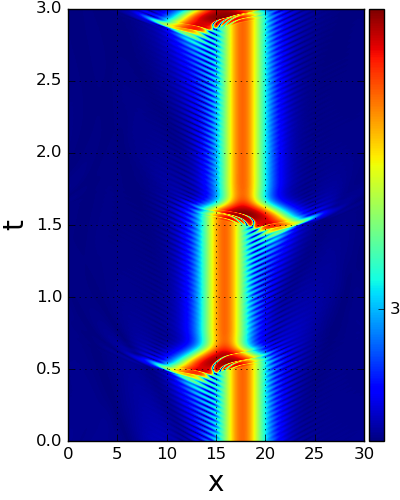
\includegraphics[width=\textwidth]{cglETDphase1}
  \end{minipage}
  \begin{minipage}{.25\textwidth}
    \centering \small{\texttt{(b)}}
    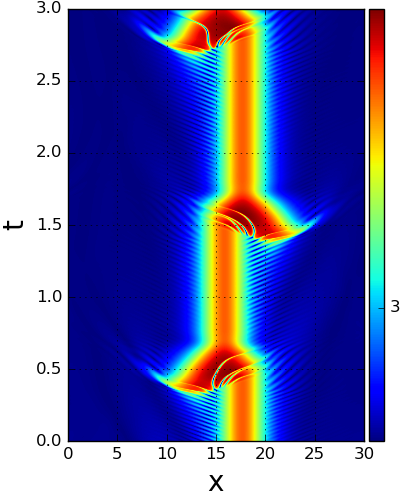
\includegraphics[width=\textwidth]{cglETDphase2}
  \end{minipage}%
  \begin{minipage}{.25\textwidth}
    \centering \small{\texttt{(c)}}
    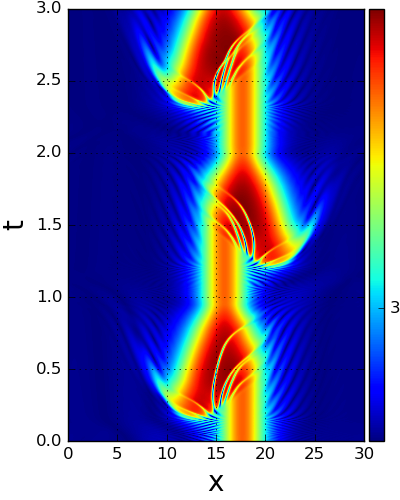
\includegraphics[width=\textwidth]{cglETDphase3}
  \end{minipage}
  \caption{ Soliton explosion profiles by Krogstad scheme :
    (a) Constant time step  $h=10^{-3}$.
    (b) Adaptive time step in static frame.
    (c) Adaptive time step in traveling frame.
  }
  \label{fig:cglETDphase}
\end{figure}

\begin{figure}[h]
  \centering
  \begin{minipage}{.32\textwidth}
    \centering \small{\texttt{(a)}}
    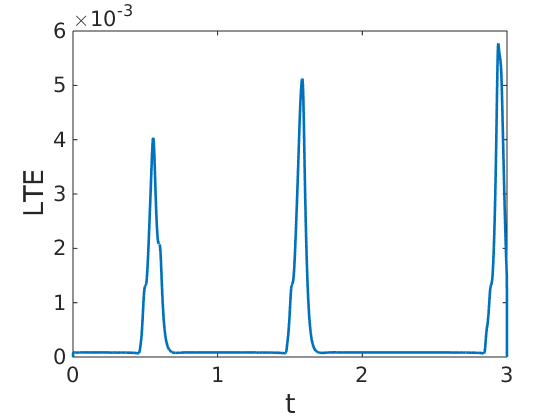
\includegraphics[width=\textwidth]{cglETDLTE1}
  \end{minipage}
  \begin{minipage}{.32\textwidth}
    \centering \small{\texttt{(b)}}
    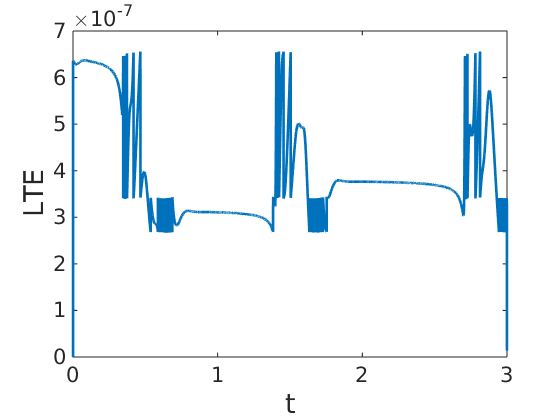
\includegraphics[width=\textwidth]{cglETDLTE2}
  \end{minipage}%
  \begin{minipage}{.32\textwidth}
    \centering \small{\texttt{(c)}}
    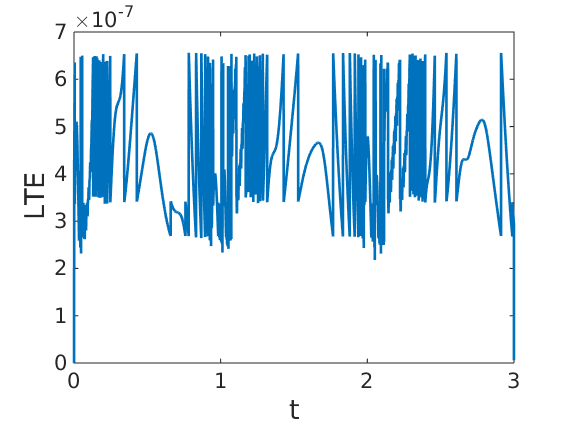
\includegraphics[width=\textwidth]{cglETDLTE3}
  \end{minipage}
  \caption{ Estimated local truncation error by Krogstad scheme :
    (a) Constant time step $h=10^{-3}$.
    (b) Adaptive time step in static frame.
    (c) Adaptive time step in traveling frame.
  }
  \label{fig:cglETDLTE}
\end{figure}

\begin{figure}[h]
  \centering
  \begin{minipage}{.4\textwidth}
    \centering \small{\texttt{(a)}}
    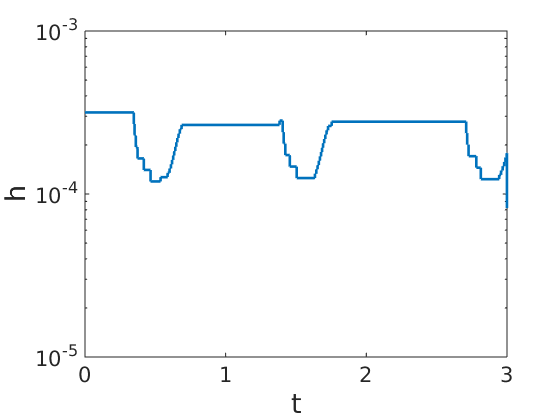
\includegraphics[width=\textwidth]{cglETDh2}
  \end{minipage}
  \begin{minipage}{.4\textwidth}
    \centering \small{\texttt{(b)}}
    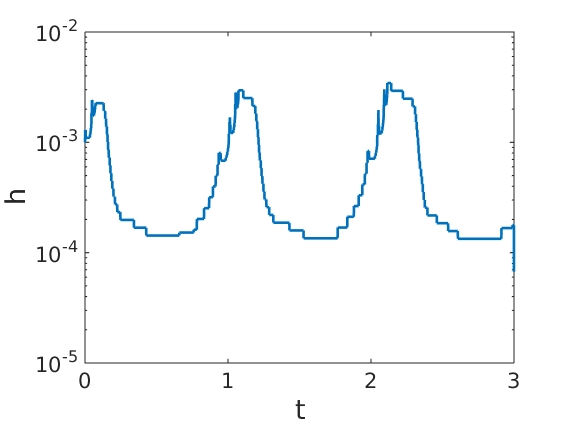
\includegraphics[width=\textwidth]{cglETDh3}
  \end{minipage}%
  \caption{ Time step used during integration by Krogstad scheme :
    (a) Adaptive time step in static frame.
    (b) Adaptive time step in traveling frame.
  }
  \label{fig:cglETDh}
\end{figure}

\begin{table}[h]
  \centering
  \begin{tabular}{c  c c  c c}
    & \multicolumn{2}{c}{ETDRK4} & \multicolumn{2}{c}{Krogstad} \\
    \hline
    &  TA & TATF & TA & TATF \\
    NReject &  51 & 86 & 51 & 108 \\
    NevaCoe &  87 & 141 & 87 & 178 \\
    Ns & 12532 & 4653 & 12581 &  4544 \\
    \hline
  \end{tabular}
  \begin{tabular}{l l }
    & \\
    TA  &  Time adaptive scheme \\
    TATF &  Time adaptive in traveling \\
         & frame scheme \\
    NRject &  number of time the calculated \\
           &  new state is rejected due to large \\
           &  estimated local truncation error  \\
    NevaCoe &  number of time to recalculate Butcher table \\
    Ns & number of integration steps \\
  \end{tabular}
  \caption{
    Compassion between ETDRK4 and Krogstad.
  }
  \label{tab:ETDKrog}
\end{table}

As an experiment, we test the performance of the time step adaptive ETDRK4 and
Krogstad in one dimensional \cqcGLe.
In a certain range of parameters, this system exhibits intermittent
explosion. So the dynamics of this system has two different time scales :
every slow movement around a relative equilibrium  and
every fast burst when the soliton explodes. We anticipate the time step adaptive
ETDRK4 and Krogstad can slow down at the explosion part and accelerate at the
slow part.

In the experiments, we set the integration time period to be $[0, 3]$ and the
relative error tolerance $\epsilon=10^{-6}$. The constant time step schemes use
time step $h=10^{-3}$. All tests use the same initial condition.

\refFig{fig:cglETDphase} (a)(b) show the evolution of $|A|$ using
constant time step and adaptive time step Krogstad method respectively.
During the integration period, three explosion instances are observed. The
explosion parts in (b) are stretched a little bit compared with (a) because the
time adaptive scheme slows down during explosion parts.
\refFig{fig:cglETDLTE} (a)(b) are the corresponding estimated local truncation
error during the same period. Without local error control, the constant time step
Krogstad has bad performance for the explosion part, during which local truncation
error reaches as large as $6\times 10^{-3}$. While local truncation
error is controlled under $10^{-6}$ for time step adaptive scheme.

However, as shown in \reffig{fig:cglETDh}(a) the time step adaptive Krogstad
method still uses every small time step ($\sim 3\times 10^{-4}$)
even for the slow motion part. In fact, the stiffness actually comes from fast phase
rotation of complex field $A$. Until now, we are only interested in the magnitude
of field $A$ and turn a blind eye to its phase. However, orbits of this system in
the state space is circulating around a relative equilibrium of the form
\[
  A_0(t, x) = A_0(x)e^{i\omega_0 t}
  \,
\]
with phase rotating velocity $\omega_0 =176.675049$ a very large number. Thus dynamics
close to this relative equilibrium will have similar large phase rotation.
Therefore, we integrate the system in a traveling frame by setting
\[
  A(x, t) = \tilde{A}(x, t)e^{i\omega_0 t}
\]
The dynamics of $\tilde{A}(x, t)$ is shown in \reffig{fig:cglETDphase}(c). The
corresponding local truncation error and time steps are shown in
\reffig{fig:cglETDLTE} and \reffig{fig:cglETDh} respectively. We can see that
time step used in this traveling frame is almost one order larger that that in the
static frame for the slow motion part. But for the explosion part, both use time
step $\sim 10^{-4}$.

Time step adaptive ETDRK4 is also tested and the result is compared with
Krogstad method in \reftab{tab:ETDKrog}. The difference between these two
methods are minimal. Since ETDRK4 has more empty locations in its Butcher
table, evaluation of Butcher table is more efficient in ETDRK4 than Krogstad.
So, in practice, we prefer to use adaptive ETDRK4 to integrate \cqcGLe.
\refTab{tab:ETDKrog} also shows that integration in the traveling frame is
much more efficient than in the static frame.

\paragraph{Some notes}
For record purpose, I list the coefficients of Butcher table in
ETDRK4 and Krogstad for easy implementation.
\begin{itemize}
\item ETDRK4
  \[
    E = e^{hL}\,,\quad 
    E_2 = e^{hL/2}\,,\quad
    a_{21} = \frac{e^{hL/2}-1}{L}
  \]
  \begin{align*}
    b_1 & = h^{-2}L^{-3}[-4-hL+e^{hL}(4-3hL+(hL)^2)] \\
    b_2 = b_3 & = 2h^{-2}L^{-3}[2+hL+e^{hL}(-2+hL)] \\
    b_4 & = h^{-2}L^{-3}[-4-3hL-(hL)^2+e^{hL}(4-hL)] \\
  \end{align*}
  \begin{align*}
    U_1 & = u_n \\
    U_2 & = E_2 u_n + a_{21} \mathcal{N}(t_n, u_n) \\
    U_3 & = E_2 u_n + a_{21} \mathcal{N}(t_n+\frac{h}{2}, U_2) \\
    U_4 & = E_2 U_2 + a_{21} (2\mathcal{N}(t_n+\frac{h}{2}, U_3)-
          \mathcal{N}(t_n, u_n) )\\
    U_5 & = E u_n + b_{1} \mathcal{N}(t_n, u_n)
          +b_2[\mathcal{N}(t_n+\frac{h}{2}, U_2) + 
          \mathcal{N}(t_n+\frac{h}{2}, U_3)]
          +b_4 \mathcal{N}(t_n+h, U_4) )\\
    u_{n+1} & = U_5
  \end{align*}
  A trick is used in $U_4$.

\item Krogstad scheme.
  $E$, $E_2$, $a_{21}$, $b_1$, $b_2$ $b_3$ and $b_4$ are the same as 
  ETDRK4.
  Other coefficients are 
  \[
    a_{31} =  h^{-1}L^{-2}[4+hL+e^{hL/2}(hL-4)]\,,\quad 
    a_{32} =  2h^{-1}L^{-2}[-2-hL+2e^{hL/2}]
  \]
  \[
    a_{41} =  h^{-1}L^{-2}[2+hL+e^{hL}(hL-2)]\,,\quad 
    a_{43} =  2h^{-1}L^{-2}[-1-hL+e^{hL}]
  \]
  \begin{align*}
    U_1 & = u_n \\
    U_2 & = E_2 u_n + a_{21} \mathcal{N}(t_n, u_n) \\
    U_3 & = E_2 u_n + a_{31} \mathcal{N}(t_n, u_n) +
          a_{32} \mathcal{N}(t_n+\frac{h}{2}, U_2) \\
    U_4 & = E_2 u_n + a_{41}\mathcal{N}(t_n, u_n) 
          + a_{43}\mathcal{N}(t_n+\frac{h}{2}, U_3) \\
    U_5 & = E u_n + b_{1} \mathcal{N}(t_n, u_n)
          +b_2[\mathcal{N}(t_n+\frac{h}{2}, U_2) + 
          \mathcal{N}(t_n+\frac{h}{2}, U_3)]
          +b_4 \mathcal{N}(t_n+h, U_4) )\\
    u_{n+1} & = U_5
  \end{align*}
\end{itemize}

%%%%%%%%%%    end of the differential matrix part     %%%%%%%%%%%%%%%%%%%%%%%%%%%%
